\documentclass{article}
  \parindent = 0mm % Sin sangría
  \usepackage[utf8]{inputenc}
  \usepackage[T1]{fontenc}
  \usepackage[spanish]{babel}
  \usepackage{graphicx}
  \usepackage{amstext}
  \usepackage{amsmath}
  \usepackage{booktabs}
  \usepackage{subfigure}
  \usepackage{footnote}
  \usepackage{hyperref}
  \usepackage{algpseudocode,algorithm,algorithmicx}
  \usepackage[font=small,labelfont=bf]{caption}

\begin{document}
  \begin{center}
    {\sc \large Enfoque de pulsos}
    
    {\sc \large Proyecto 2020}
    \linebreak

    {\rm Joaquín Correa - \today}
  \end{center}

  \section*{Introducción}

  Como proyecto de aplicación del algorítmo del Pulso se propone su aplicación al problema de ruteo de demanda y decisión de construcción de ciclovías en una ciudad, puede ser visto como una versión del problema de distribución de mercancías, sobre una red que puede ser modificada mediante la construcción de instalaciones que mejoren la distribución. Se utiliza el pulso como método alternativo a la programación matemática con el objetivo de escalar mejor en el tamaño de las instancias atacables, aunque con esto se pueda perder la óptimalidad, es decir lo utilizo como metaheurístca. Finalmente se realiza un comparación en medida de lo posible con el MILP que resuelve el problema exacto e incluyo una sección con características propias y trabajo futuro.

  \section*{Problema}

  El problema consiste en decidir dónde construir ciclovías de manera que satisfaga las necesidades de los usuarios, representados por la demanda, de la mejor manera. Matemáticamente, el modelo consiste en un grafo dirigido y un conjunto de pares origen-destino donde para cada uno se tiene un valor de demanda (por ejemplo cantidad de personas). Para cada arco del grafo, se tiene un costo de usuario que corresponde al costo percibido por un usuario si lo utiliza para desplazarse y un costo de construcción de diversos tipos de ciclovías. Al construir una ciclovía sobre un arco, el costo de usuario disminuye frente a la no construcción. Finalmente se tiene un valor de presupuesto que limita la construcción de ciclovías.

  La formulación matemática es la siguiente:

  \begin{align}
    \text{min} & \sum_{k \in O} \sum_{i \in I} \sum_{e \in E} x_{ek}^i c_e^i & \label{eq:objective} \\
    \text{s.t.} & \sum_{i \in I}\sum_{e \in E_n^+} x_{ak}^i - \sum_{i \in I}\sum_{e \in E_n^-} x_{ak}^i = b_{nk} & \forall k \in O, n \in V \label{eq:flowconservation} \\
          & \sum_{i \in I} y_{e}^i \leq 1 & \forall e \in E \label{eq:onlyoneinfraactive} \\
          & \sum_{i \in I} \sum_{e \in E} m_e^i y_e^i \leq B & \label{eq:respectbudget} \\
          & x_{ek}^i \leq y_e^i  D_k & \forall e \in E, i \in I, k \in O \label{eq:restrictflowbyinfras} \\
          & x_{ek}^i \geq 0, y_e^i \in \{0,1\} &
  \end{align}

  Donde:
  \begin{description}
    \item[$O$]: Conjunto de pares origen-destino.
    \item[$I$]: Conjunto de infraestructuras.
    \item[$G=(V, E)$]: Grafo dirigido, compuesto por el conjunto de vértices $V$ y arcos $E$.
    \item[$c_e^i$]: Parámetro, costo de usuario de atravesar el arco $e$ utilizando la infraestructura $i$.
    \item[$b_{nk}$]: Parámetro, valor de la ecuación de conservación del flujo. Vale $D_k$ si $n$ es el origen de $k$, $-D_k$ si es el destino y cero en otro caso.
    \item[$m_e^i$]: Parámetro, costo de construcción de la infraestructura $i$ sobre el arco $e$.
    \item[$B$]: Parámetro, valor del presupuesto total de construcción.
    \item[$x_{ek}^i$]: Es la variable que modela el flujo de demanda del par origen-destino $k$, sobre el arco $e$ utilizando la infraestructura $i$.
    \item[$y_e^i$]: Es la variable binaria que indica si la infraestructura $i$ está activa en el arco $e$.
  \end{description}

  Y las ecuaciones:

  \begin{description}
    \item[(\ref{eq:objective})] Objetivo, se minimiza el costo total percibido por el flujo.
    \item[(\ref{eq:flowconservation})] Restricción de conservación del flujo.
    \item[(\ref{eq:onlyoneinfraactive})] Restricción que permite solo una infraestructura activa por arco.
    \item[(\ref{eq:respectbudget})] Restricción de presupuesto.
    \item[(\ref{eq:restrictflowbyinfras})] Restricción que permite al flujo utilizar la infraestructura activa únicamente.
  \end{description}

  \subsection*{Modelado}

  Se puede observar de la formulación, que si bien el grafo base es un grafo simple, se está trabajando sobre un multigrafo. Cada arco del grafo base es replicado tantas veces como cantidad de infraestructuras hay y cada replica tiene un costo de usuario y costo de construcción asociado.

  Lo que se busca son caminos óptimos por este multigrafo, con restricción de presupuesto. Notar que si se activa la infraestructura $i$ en el arco $e$, esta puede ser usada por cualquiera de los flujos entre pares origen-destino.

  Una cosa que no esta representada en el modelo, pero que se desprende de la realidad, es que siempre habrá una solución factible. Esto es debido a que se toma el grafo base como una de las infraestructuras cuyo costo de construcción es cero.

  \subsection*{Dificultades}

  Este problema, asi como fué formulado puede resolverse en un MILP solver para grafos no muy grandes de manera conveniente. Pero, al ser en parte un problema de programación entera sabemos es un problema contenido en $NP$ y por lo tanto, todavía, difícil de escalar.

  Particionando el problema en dos, con el solo objetivo de analizarlo, por un lado esta la decisión de cuál y dónde construir infraestructura y por otro la de encontrar el camino más corto para cada par origen-destino. La primera partición del problema es la difícil, la segunda, vista de manera aislada es un problema {\it fácil}: el flujo entre dos pares origen destino no esta relacionado con otros flujos, ni los arcos tienen capacidad. Por lo tanto, la segunda partición es simplemente el problema del camino mas corto entre dos puntos, repetido $card(O)$ veces. Lo que se busca en este trabajo, es utilizar el pulso para resolver ambos problemas al mismo tiempo.

  \section*{Aplicación del Pulso}

  Supongamos para simplificar, que tenemos un único par origen-destino. Debemos encontrar la asignación de infraestructuras a arcos que hagan mejor uso del presupuesto $B$. Si modelamos el grafo con infraestructuras como un multigrafo, esto se puede resolver como un problema de camino más corto con restricciónes o weighted-constrained shortest-path. Aquí es donde entra el algorítmo del Pulso.

  Es de suponer, que en la simplificación de un único par origen-destino, el pulso, o cualquier algorítmo exacto para el WCSP debe encontrar la mejor solución, la misma que encontraría el MILP solver. Sin embargo, si consideramos mas de un par origen-destino el problema se complejiza.

  Si bien los pares origen-destino son independientes, la red subyacente es común, y el hecho de que una infraestructura esté activa o no en cierto arco puede determinar el camino mas corto entre varios pares origen-destino. Supongamos que se toma un par origen-destino y se ejecuta el pulso con cierta restricción de presupuesto. Luego se toma el siguiente par origen-destino y se ejecuta el pulso, con cierta restricción de presupuesto, si es que aún queda, y sobre el multigrafo luego de aplicar las infraestructuras que el pulso eligió para el primer par origen-destino. Se puede continuar este proceso iterativo hasta quedarse sin pares origen-destino. El hecho de quedarse sin presupuesto no afecta en lo mas mínimo, debido a que siempre habrán caminos cuyos costo de construcción sean cero. A grandes rasgos, este fue el camino que se siguió.

  Lo que queda por definir es la asignación de presupuesto para cada ejecución del pulso. Se decidió asignar a cada origen-destino la proporción de presupuesto relativa a la demanda de dicho par sobre el total, es decir: el presupuesto del par $k$ es $B_k = B  {D_k \over \sum_{s \in O} D_s}$.

  \subsection*{Consideraciones del pulso}

  Se implementó una versión del pulso simple que incluye las siguientes características:

  \begin{description}
    \item[Poda por costo]: {se corre inicialmente un Dijkstra sobre el reverso del grafo base\footnote{El grafo con los arcos en sentido opuesto}, para obtener una cota inferior del costo desde cada nodo al nodo objetivo, en adelante se le referirá como {\it cost bound}. Luego se utiliza esta información para realizar la poda por costo.}
    \item[Poda por infactibilidad]: {se corre, para cada restricción, un Dijkstra sobre el grafo reverso tomando dicha restricción como el costo de los arcos. De esta forma obtenemos un valor mínimo de cada restricción requerido para llegar al nodo destino.}
    \item[Poda por dominancia]: {cuando un pulso llega a un nodo, se verifica que dicho pulso no esté dominado por algún otro pulso que ya se encuentre en el nodo.}
    \item[Cola de pulsos]: {En cada iteración, el pulso elegido es el que tiene menor costo proyectado. Es decir, cuyo costo actual mas la cota inferior del costo en el nodo, es menor.}
  \end{description}

  \subsection*{Modos de ejecución}

  \subsection*{Pulse Solver}

  El algoritmo que soluciona el problema, llamémoslo {\it Pulse solver}, se implementó como un algoritmo recursivo que en cada paso recursivo selecciona un par origen destino, corre el pulso y para cada camino generado, lo aplica al grafo, llama al paso recursivo y luego vuelve el grafo a su estado anterior. El solver puede tener una cantidad exponencial (en la cantidad de pares origen-destino) de pasos recursivos, si el pulso genera muchos caminos en cada paso. Por eso necesario que cada camino generado por el pulso sea lo mejor posible. Más allá de los caminos que pueda generar el pulso en cada paso, se puede limitar la cantidad considerada con un parámetro del programa.

  Cada ejecución del árbol de recursiones es considerada una iteración. Se puede configurar la cantidad de iteraciones a realizar el algorítmo. En cada iteración, la secuencia en que son elegidos los pares origen destino es aleatorizada.

  Para flexibilizar un poco el presupuesto asignado a cada pulso, se pueden especificar dos numeros $P_{\alpha}$ y $P_{\beta}$ de manera que el presupuesto asignado al par origen destino $o$, sea $BP_oP_{\alpha} + P_{\beta}$, donde $P_o$ es la proporción del total del presupuesto total $B$ asignado a $o$. Esto puede causar que los últimos pares origen-destino considerados en la recursión tengan presupuesto $0$, pues este se asigno completamente a pares origen-destino anteriores en la recursión.

  \subsection*{Pulso}

  El algoritmo del pulso requiere cuatro parámetros en su forma mas básica: el grafo, las restricciones y los nodos origen y destino. Se implementó de manera que sea mas bien un generador de caminos entre los nodos origen y destino. Para limitar la cantidad de caminos generados se puede incluir un parámetro que indica el costo máximo que deben tener los caminos generados y también existe la posibilidad de que devuelva unicamente el mejor. Estos últimos parámetros son de utilidad ya que la complejidad de buscar la mejor solución es mucho mayor que buscar una solución suficientemente buena, como se describirá en la sección de resultados.

  \subsection*{Otras opciones}

  \begin{description}
    \item[Descartar nodos mas lejanos:] Booleano, por defecto falso. Durante la ejecución del pulso, no considera nodos cuya cota mínima de costo sea mayor a la del pulso corriente. Esto puede ser deseado o no dependiendo del conjunto de datos.
    \item[Delta de descarte de nodos mas lejanos:] Número, valor de la diferencia a partir del cual se descartan nodos mas lejanos. También puede ser usado para forzar la elecciones de nodos mas cercanos, si se utiliza un valor negativo.
  \end{description}

  \section*{Casos de estudio}

  En esta sección se comparan los tiempos y las variables obtenidas de la ejecución del solver GLPK\footnote{Gnu Linear Programing Kit} y el Pulse solver. Sobre el último, se detallará para cada caso la configuración utilizada.

  GLPK es ejecutados con la opción de utilizar métodos de Cutting-Plane, lo que mejora considerablemente su tiempo de ejecución frente al Branch and Cut.

  \subsection*{Ciudad Vieja}

  El primer caso de comparación y ejecución del modelo se realizó con un grafo que representa aproximadamente\footnote{Se generó a partir de información de cruces de calles} el barrio Ciudad Vieja de Montevideo. En este grafo todas las calles van en ambas direcciones. Cuenta con 204 nodos y 770 arcos y su inexacta representación esta en la figura.

  \begin{figure}[h!]
    \centering
    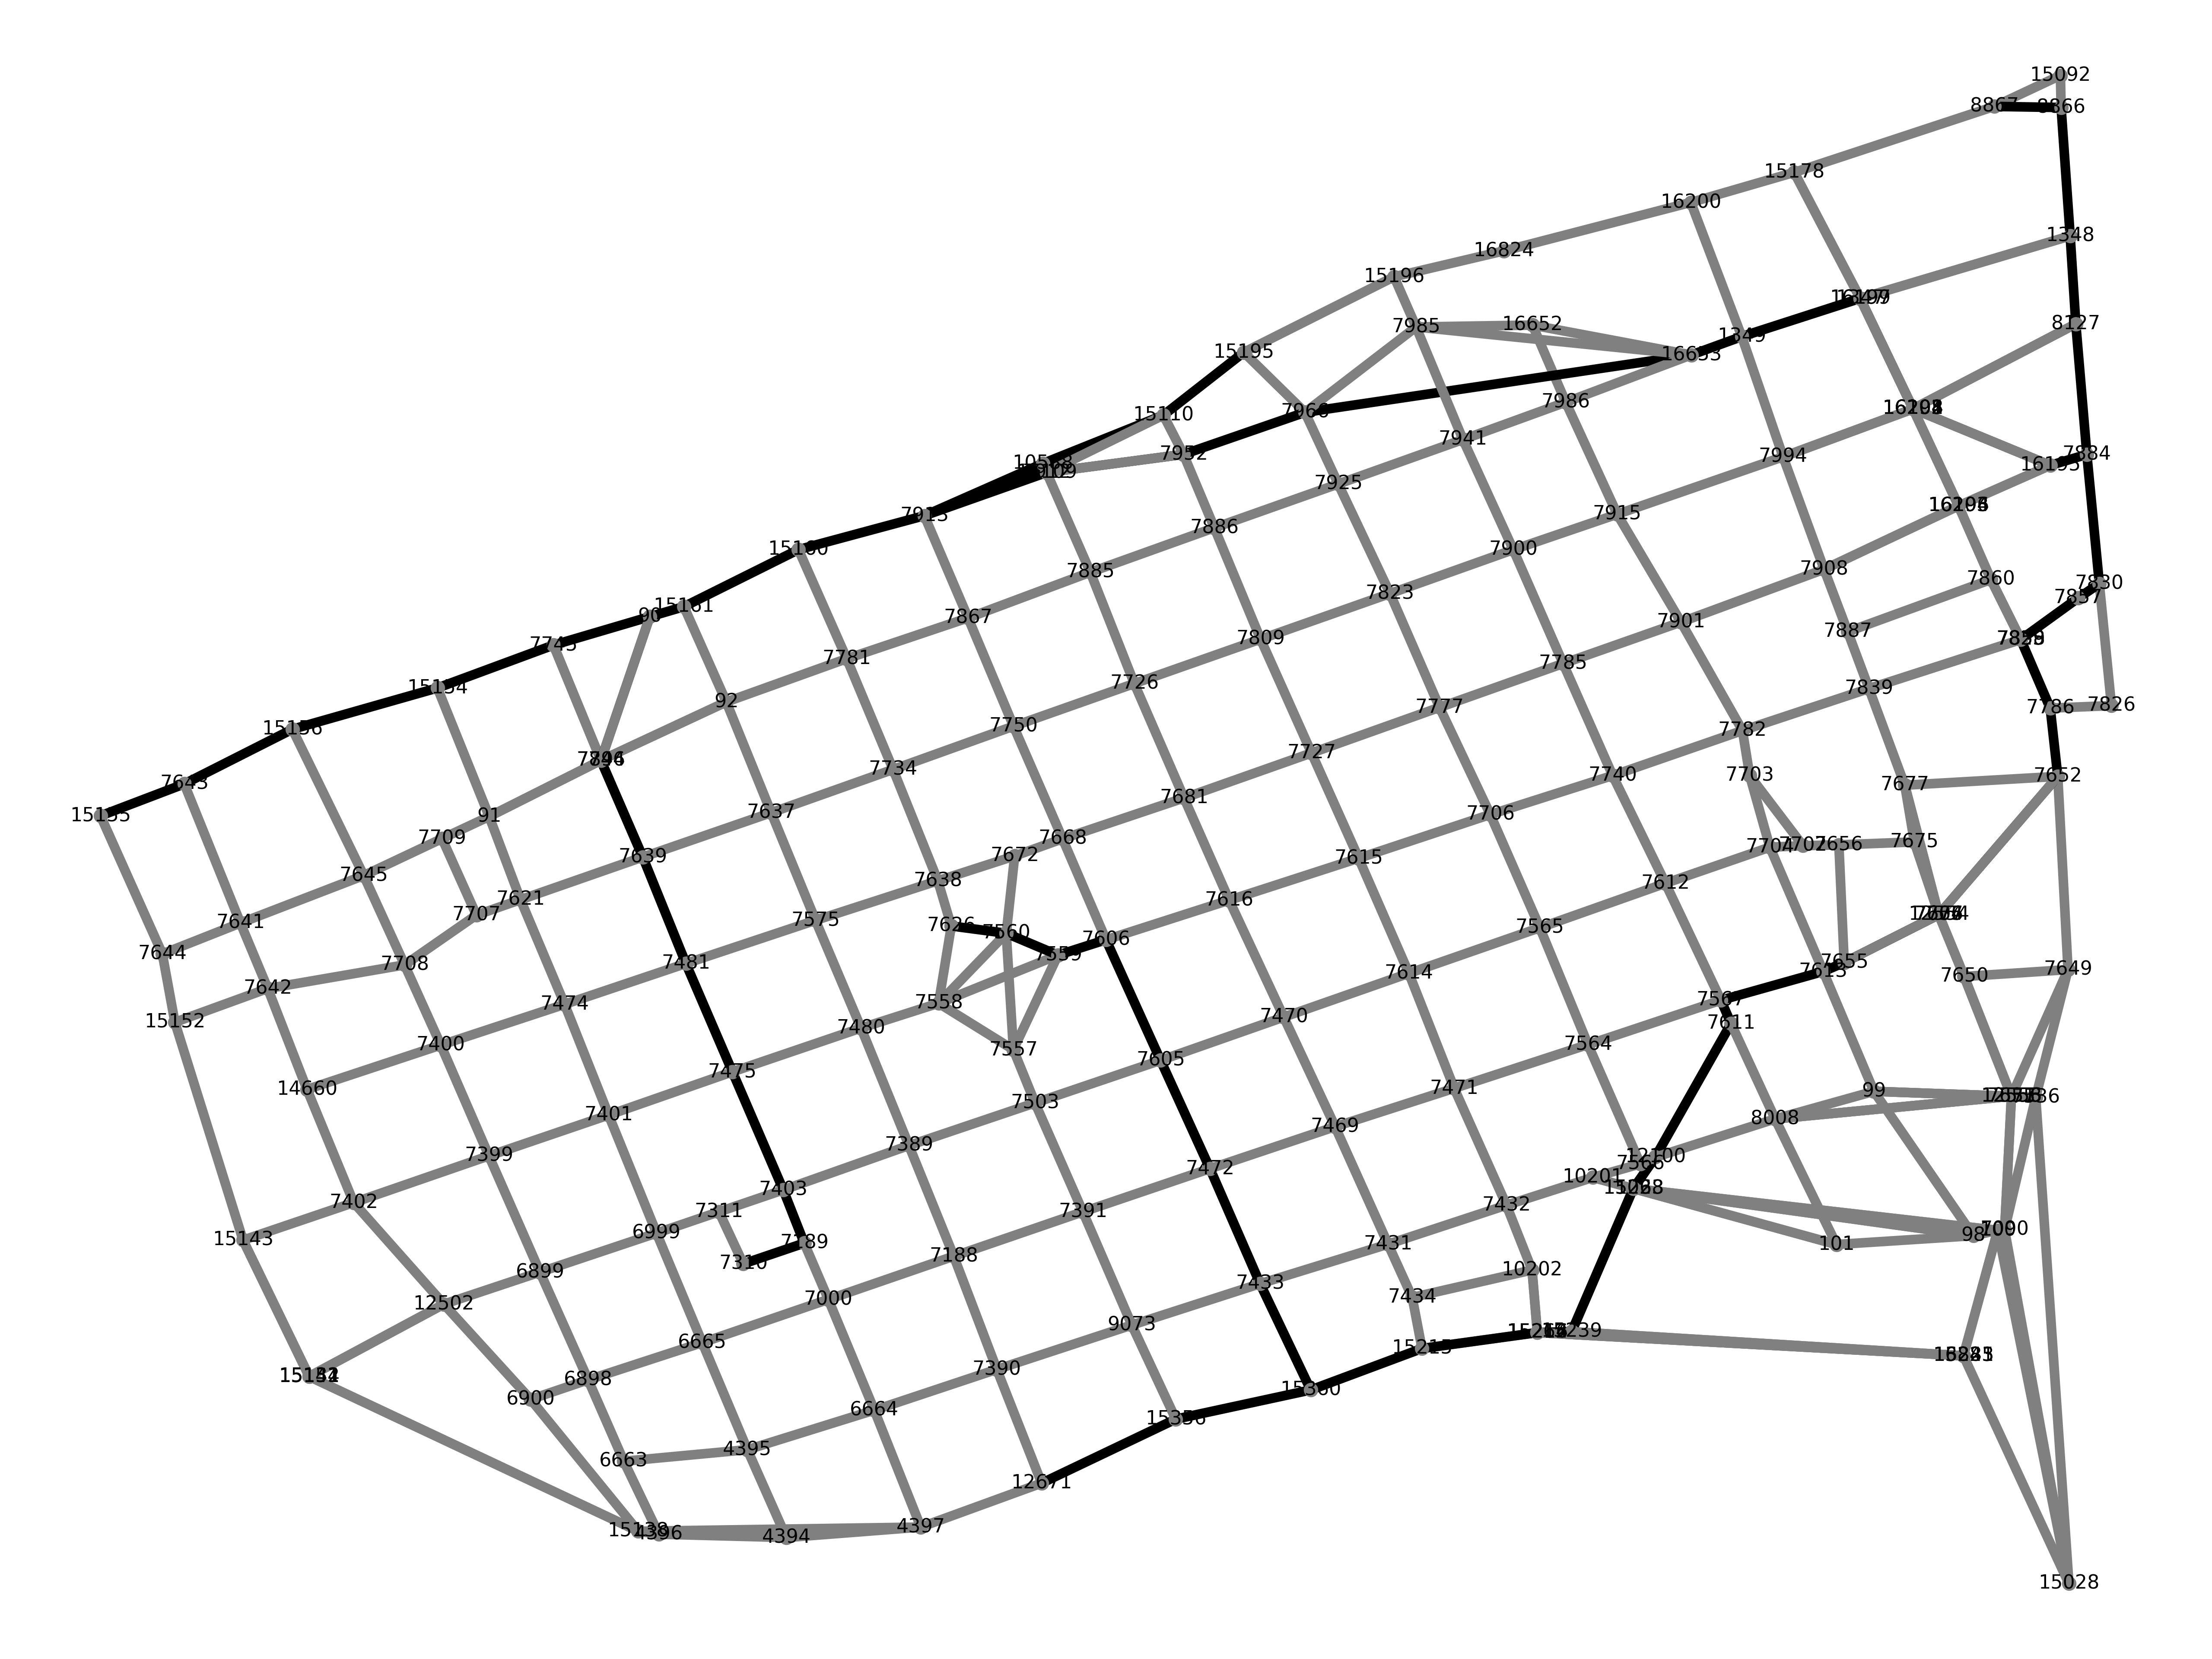
\includegraphics[width=6cm]{imgs/mdeo_med_base.png}
    \caption{Grafo de Ciudad Vieja, 204 nodos y 770 arcos. Los arcos negros marcan el camino más corto sobre el grafo base entre los cuatro pares origen destino. Notar que estos caminos pueden estar cortados ya que hay arcos solapados debido a errores en la generación del grafo base, lo que causa que el arco pintado de negro quede debajo del gris.}
    \label{ciudadvieja}
  \end{figure}

  Para este caso de prueba, se eligieron cuatro pares origen destino y un presupuesto de 15.000. En la tabla \ref{table:odsciudadvieja} se pueden observar los pares origen-destino elegido y el costo del camino mas corto sobre el grafo base. El valor objetivo en el grafo base, es decir suma del costo percibido por la demanda por el camino más corto de cada una en el grafo base, es de 1.496.098,44.

  \begin{table}[h!]
    \centering
    \begin{tabular}{ccc}
      \toprule
      Par OD & Demanda & Mejor costo base \\
      \midrule
      0 & 500 & 1585,97 \\
      1 & 50 & 1078,17 \\
      2 & 100 & 713,04 \\
      3 & 250 & 1651,14 \\
      \bottomrule
    \end{tabular}
    \caption{Resumen de pares origen-destino considerados para Ciudad Vieja. Estos datos de fueron elegidos de forma manual.}\label{table:odsciudadvieja}
  \end{table}
  
  Ademas, se especificaron tres infraestructuras construibles, que junto a la infraestructura base quedan en cuatro. Los factores de mejora y de construcción se especifican sobre el costo de usuario, en la tabla \ref{table:infrasciudadvieja}. El costo de usuario base $c$ es la distancia entre dos nodos.

  \begin{table}[h!]
    \centering
    \begin{tabular}{ccc}
      \toprule
      Infraestructura & Costo de usuario & Costo de construcción \\
      \midrule
      0 (base) & c & 0 \\
      1 & 0.9c & c \\
      2 & 0.5c & 4c \\
      3 & 0.4c & 8c \\
      \bottomrule
    \end{tabular}
    \caption{Resumen de infraestructuras consideradas para Ciudad Vieja.}\label{table:infrasciudadvieja}
  \end{table}

  Utilizando GLPK se pudo obtener una solución en poco tiempo. Por otra parte el Pulse solver requirió de muchas pruebas hasta llegar a una configuración que ejecute de manera aceptablemente rápida y encuentre una solución medianamente buena. Si utilizamos la configuración para buscar el mejor camino, entonces el tiempo de ejecución del pulse solver se dispara indefinidamente. Por otra parte se probó un factor de mejora de 0,9 que también resultó en un tiempo de ejecución excesivo, esta vez debido a que no es posible encontrar una solución que mejore en un $10\%$ el camino mas corto de uno de los pares origen-destino ya que su demanda es muy baja y por lo tanto el presupuesto asignado es insuficiente para lograr esta mejora. Luego de varias pruebas, se obtuvo un resultado medianamente bueno en tiempo de ejecución aceptable utilizando un factor de mejora de 0,97 ignorando nodos más lejanos en el pulso, un $P_{\beta}$ en el presupuesto por par origen-destino de 500, dos caminos por par origen-destino y cuatro iteraciones del solver.
  
  En la tabla \ref{table:resultadosciudadvieja} se muestra un breve resumen de los tiempos de ejecución y los valores objetivos. Luego en la figura \ref{resultadosciudadvieja} se muestran las decisiones sobre las infraestructuras tomadas por cada solver en el grafo. Se observa en la figura de representación de los resultados que la solución exacta asigna todos los recursos a las dos demandas de mayor valor, que son la que recorre el borde superior y la que recorre los bordes inferior y derecho.

  \begin{table}[h!]
    \centering
    \begin{tabular}{ccccc}
      \toprule
      Solver & Tiempo ejecución (s) & Presupuesto usado & Valor objetivo & Mejora \\
      \midrule
      GLPK  & 94,5   & 14997.77 & 763589,75 & \%49 \\
      Pulse & 106,43 & 14995.47 & 942412,85 & \%38 \\
      \bottomrule
    \end{tabular}
    \caption{Resumen de ejecución para el grafo de Ciudad Vieja. El porcentaje de mejora, es sobre el valor objetivo en el grafo base.}\label{table:resultadosciudadvieja}
  \end{table}

  \begin{figure}[h!]
    \centering
    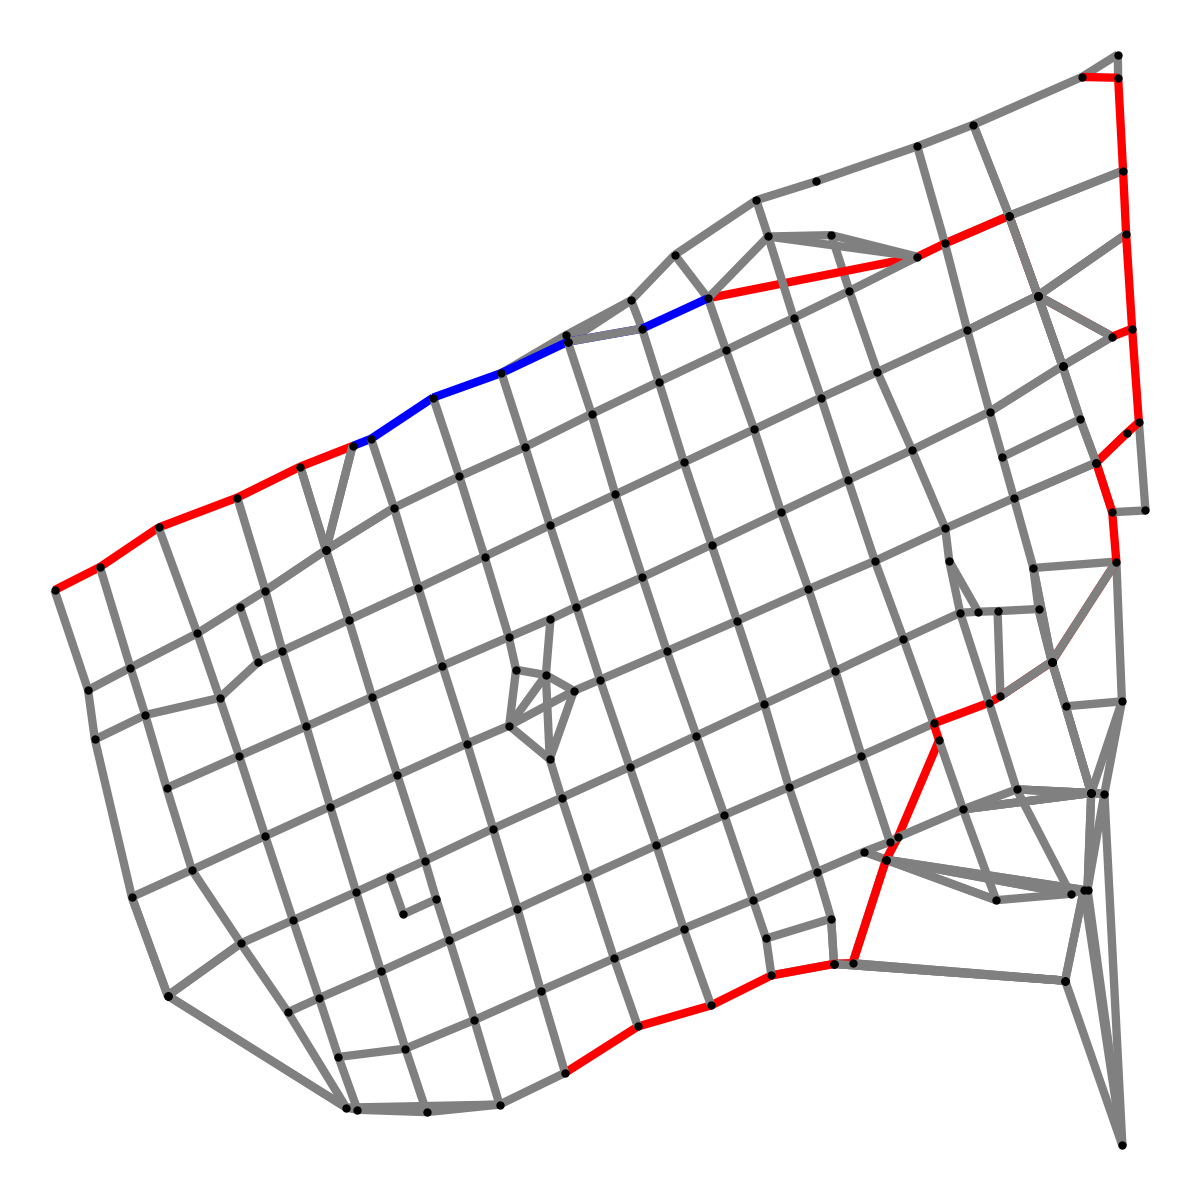
\includegraphics[width=6cm]{imgs/mdeo_med_glpk.png}
    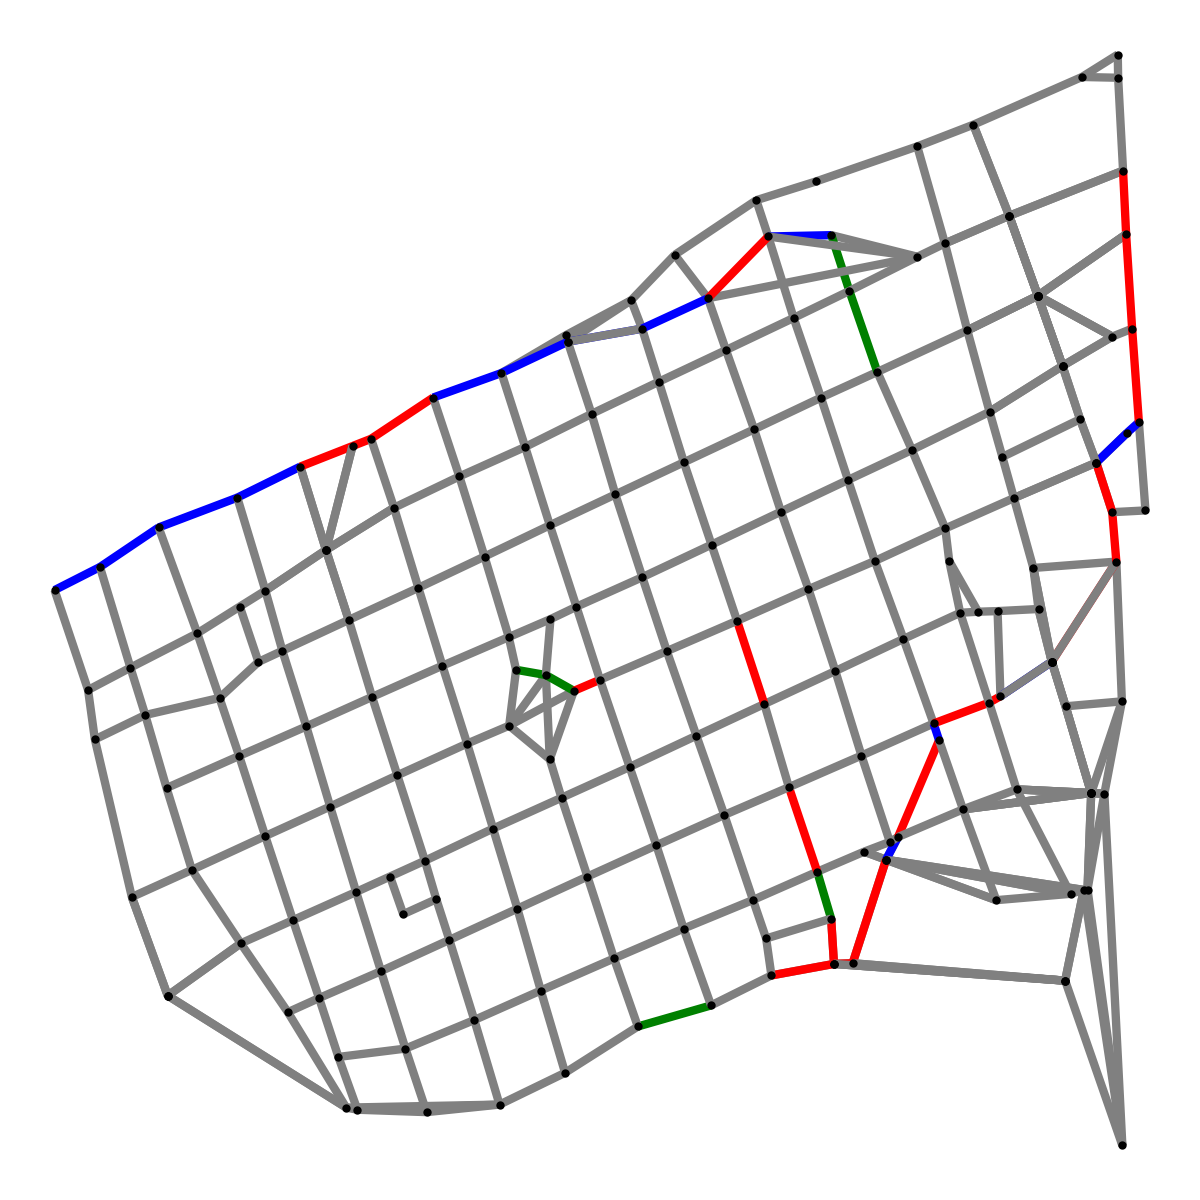
\includegraphics[width=6cm]{imgs/mdeo_med_pulse.png}
    \caption{A la izquierda las infraestructuras construidas por GLPK. A la derecha las construidas por el pulse solver. Los colores de las infraestructuras son: gris, verde, rojo y azul respectivamente al orden en que fueron definidas.}
    \label{resultadosciudadvieja}
  \end{figure}

  \subsection*{Montevideo}

  Como caso de estudio mas complejo se tomó una región más grande de la ciudad de Montevideo, la cual contiene a Ciudad Vieja. Para este grafo se eligieron cinco pares origen-destino (detallados en la tabla \ref{table:odsmontevideo}) y un presupuesto de 50.000. Las infraestructuras y sus costos son los mismas que para el caso de Ciudad Vieja.

  \begin{table}[h!]
    \centering
    \begin{tabular}{ccc}
      \toprule
      Par OD & Demanda & Mejor costo base \\
      \midrule
      0 & 1540 & 4548,58 \\
      1 & 1333 & 2158,91 \\
      2 & 218 & 2158,91 \\
      3 & 650 & 6468,50 \\
      4 & 1859 & 7112,83 \\
      \bottomrule
    \end{tabular}
    \caption{Resumen de los pares origen-destino considerados para Montevideo. Estos fueron generados aleatoriamente.}\label{table:odsmontevideo}
  \end{table}

  La representación del grafo y los caminos más cortos sobre el grafo base se pueden observar en la figura \ref{montevideo}. En este caso el valor de la función objetivo base es de 28.253.371,82.

  \begin{figure}[h!]
    \centering
    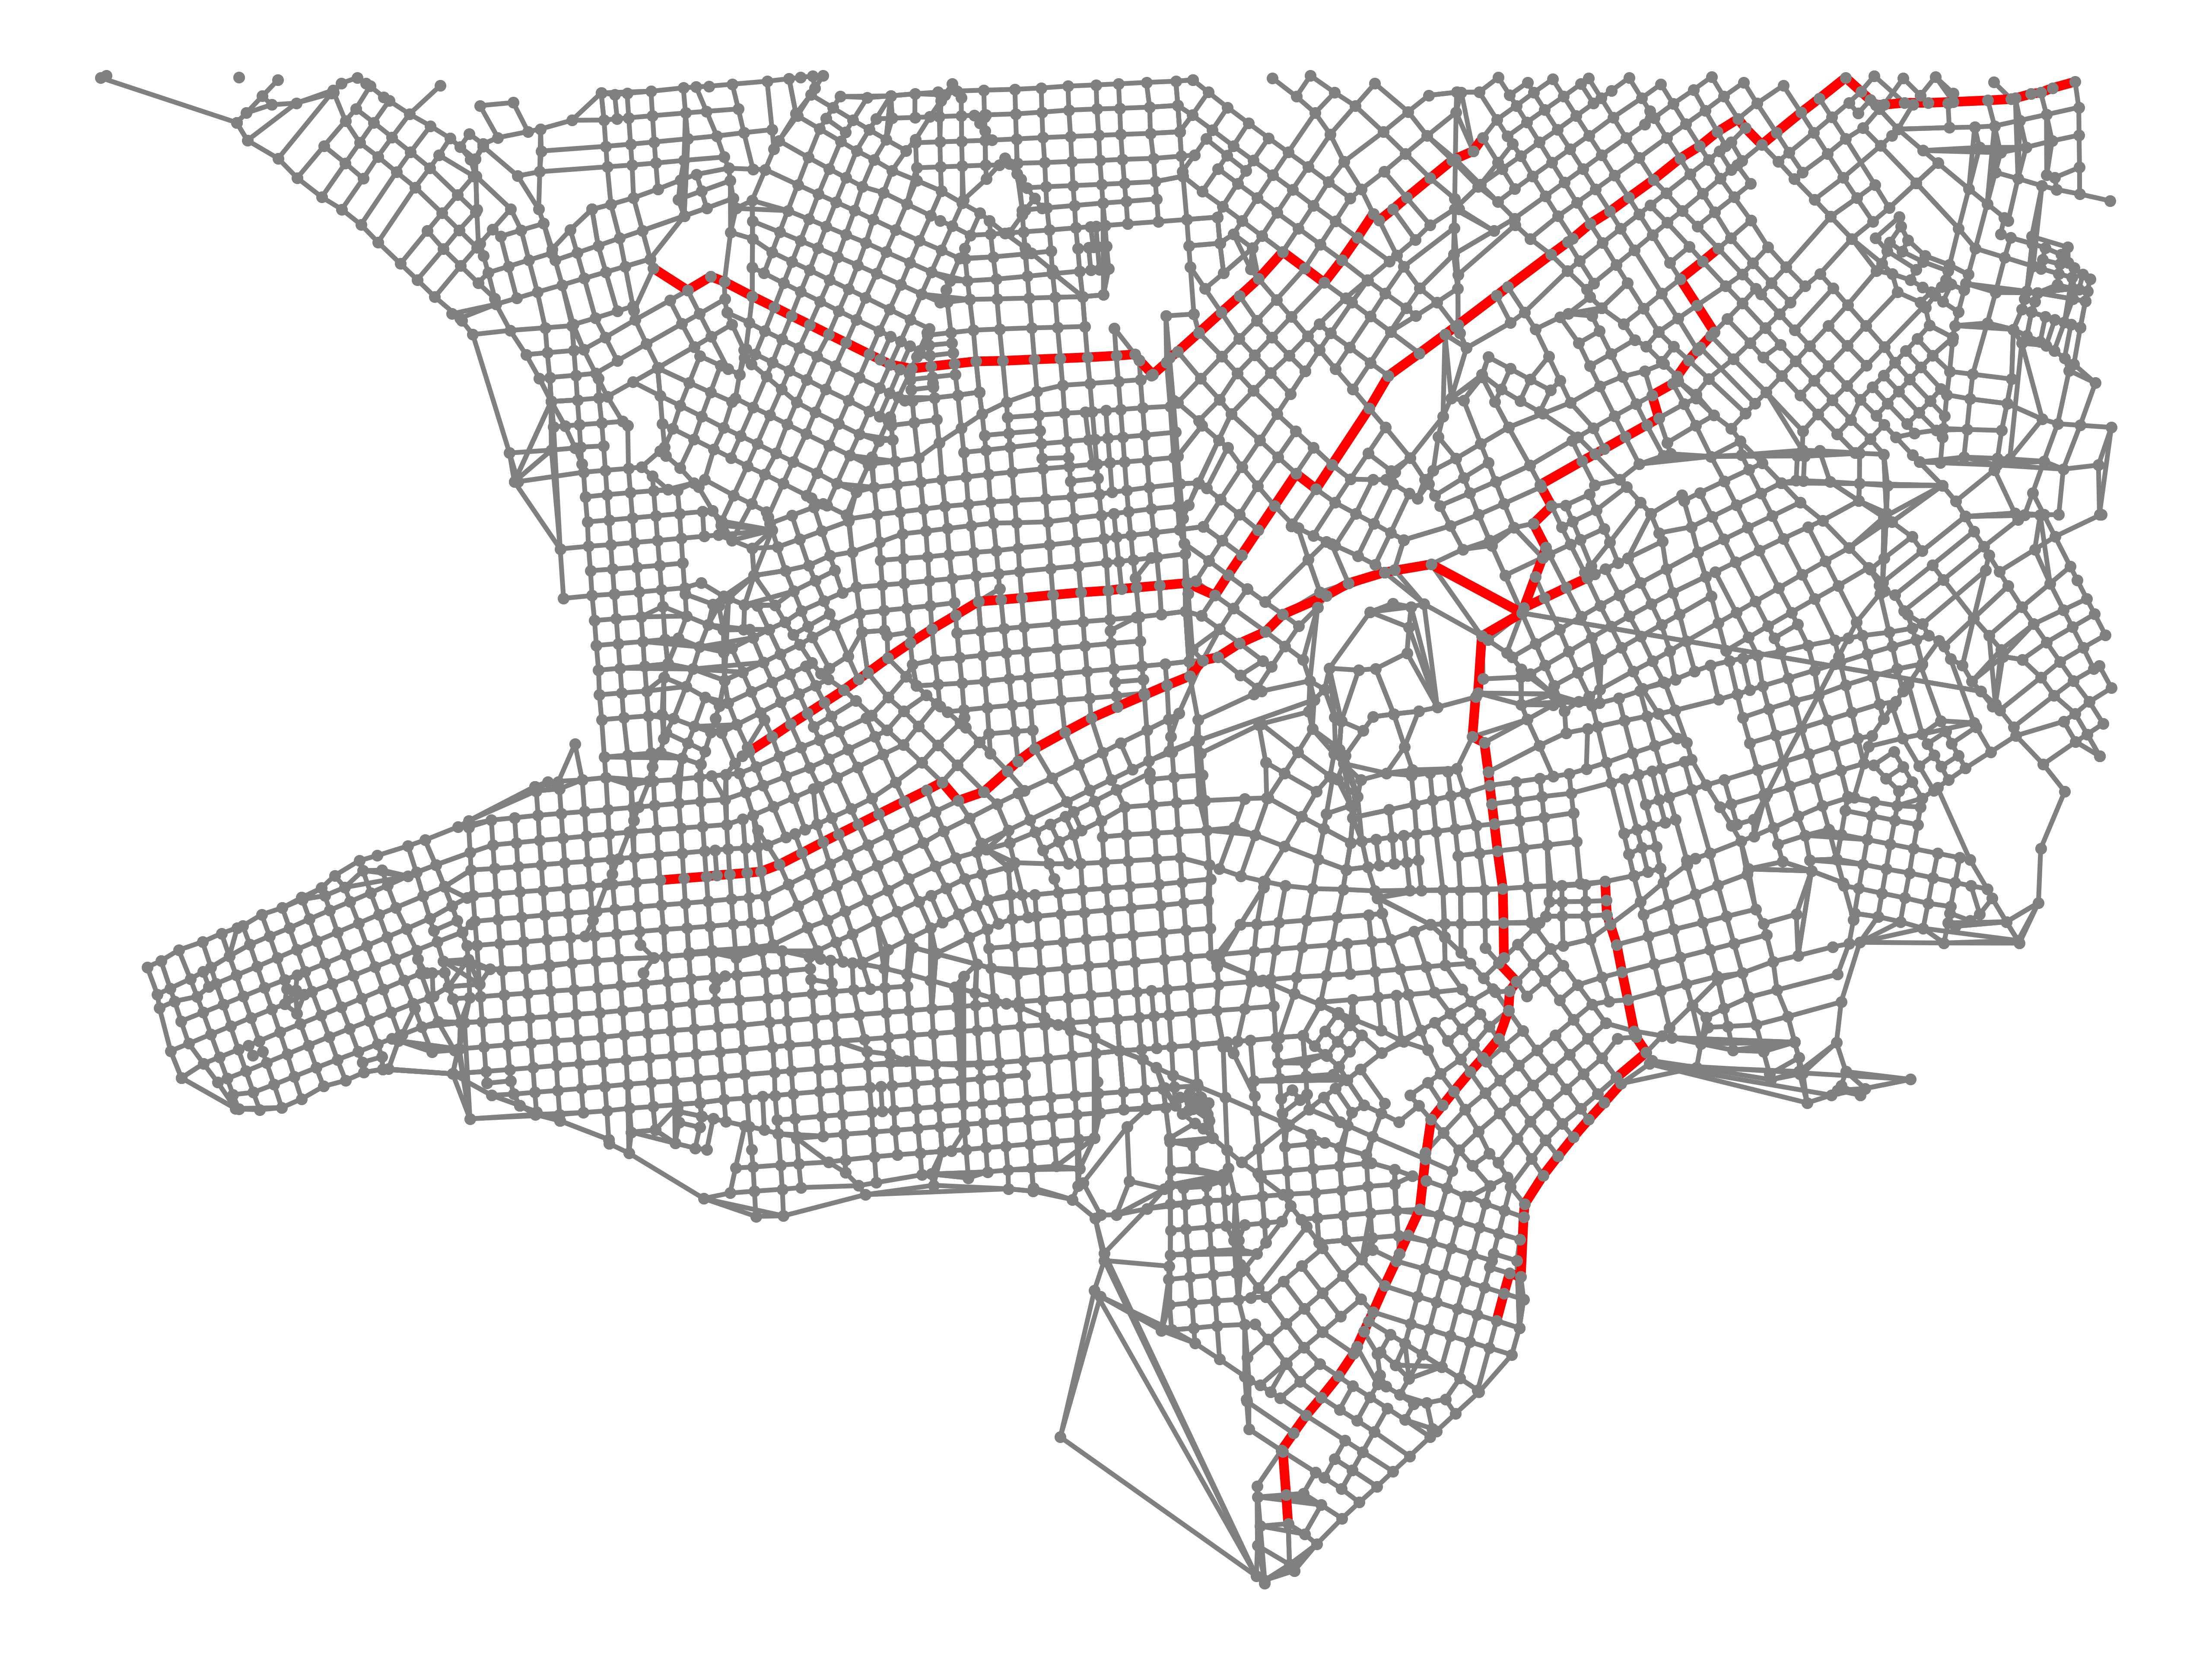
\includegraphics[width=10cm]{imgs/mdeo_large_base.png}
    \caption{Grafo de Montevideo, cuenta con 3894 nodos y 15274 arcos. Los arcos rojos marcan el camino más corto sobre el grafo base entre los pares origen destino.}
    \label{montevideo}
  \end{figure}

  La configuración para este caso fue más conservadora y se permitió solo un camino generado por par origen-destino, el hecho de que sea un grafo mucho mayor implica que el impacto de una búsqueda en espacio exponencial sea descartada. Luego se configuró un factor de mejora sobre el camino más corto base de $0.99$ y un $P_{\beta}$ de presupuesto de 300. En el pulso, como en el caso de Ciudad Vieja, se descartan nodos más lejanos.

  Durante la ejecución de este caso, se observó que el pulso tuvo dificultades para encontrar caminos a los nodos destino. Esta dificultad se vió incrementada para los pares origen-destino más lejanos en cantidad de arcos.

  Se observó que la falencia radica en la forma de ordenar la cola de pulsos. Hasta el momento, la cola de pulsos es ordenada por costo proyectado (cost bound en el nodo sumado al costo del pulso). El problema es que el cost bound, resultado de ejecutar el Dijkstra inicial, es demasiado bajo comparado con el costo que termina teniendo el camino, es decir, que no es una buena cota inferior. Esto se debe a que la mejor infraestructura tiene una disminución del costo del $60\%$, (lo que significa que el cost bound de un nodo será de $60\%$ menor que el costo sin infraestructura). Esto causa que el pulso se comporte más como un BFS que DFS. Para contrarrestar esto, se agregó una configuración: un factor que multiplique el cost bound al calcular el costo proyectado.

  Luego de varias pruebas, se determinó que un valor del factor de multiplicación del cost bound de 2,5 permite obtener resultados en tiempo aceptable para la configuración anteriormente mencionada. Este valor hace que el cost bound sea igual al costo del camino en grafo base. Valores menores al mencionado hacían que el tiempo de ejecución se dispare. Debido al corto tiempo de ejecución se pudo aumentar la cantidad de iteraciones a $20$ lo que permitió encontrar una solución un poco mejor.
  
  Durante las pruebas, diferentes valores de $P_{\beta}$ determinaban para algunos pares origen-destino que la ejecución del pulso diverja o no. Incluso luego de agregar el factor que multiplica el cost bound. Esto se observó en casos en que la asignación de presupuesto era muy baja, lo que causaba que el factor de multiplicación del cost bound sea demasiado bajo para ese caso en particular.
  
  En la figura \ref{resultadosmontevideo} se pueden observar las decisiones tomadas por el Pulse solver. Se observa claramente que las infraestructuras fueron colocadas en uno de los extremos de cada camino, lo cual indica una toma de decisiones que puede ser mejorada. El valor objetivo de esta solución es de 22.865.161,48, un $20\%$ menor que el valor objetivo en el grafo base y se obtuvo en 14 segundos.

  La ejecución en GLPK de este caso, no ha finalizado al momento de la escritura de este informe luego de 72 horas de ejecución.

  Para estimar qué tan buena es la solución encontrada, se analizó cuanto sería el valor objetivo si se construyera solo una infraestructura y se aplicara al camino más corto de cada par orgien-destino sobre el grafo base. Por ejemplo para la infraestructura 2, su costo es de 4 por cada unidad de distancia, y su beneficio es 0.5 por cada unidad de costo de usuario (que también es la distancia). Por lo tanto si solo se construye la infraestructura 2 con el presupuesto de 50.000, se pueden construir hasta ${50.000 \over 4} = 12500$ unidades de infraestructura 4. Luego para cada par origen-destino en orden descendente en cantidad de demanda, se ajustará su aporte al valor objetivo si se utilizara la infraestructura 4 en la totalidad del camino o tanto como haya disponible. El resultado para cada infraestructura se encuentra en la tabla \ref{table:montevideoestimacion}. La mejor mejora, valga la redundancia, es casi el doble que la obtenida con el Pulse solver.
  
  \begin{table}[h!]
    \centering
    \begin{tabular}{ccc}
      \toprule
      Infraestructura & Valor Objetivo & Mejora \\
      \midrule
      1 & 25475315.96 & 10\% \\
      2 & 16634621,82 & 37,8\% \\
      3 & 21282121,82 & 24,7\% \\
      \bottomrule
    \end{tabular}
    \caption{Estimación del valor objetivo si se utiliza únicamente la infraestructuras 1, o la 2 o la 3. Notar que la suma de los largos de todos los caminos más cortos de los pares origen-destino suma 22.447, por lo que si se utiliza la infraestructura 1 sobra presupuesto. El porcentaje de mejora, es sobre el valor objetivo en el grafo base.}
    \label{table:montevideoestimacion}
  \end{table}


  \begin{figure}[h!]
    \centering
    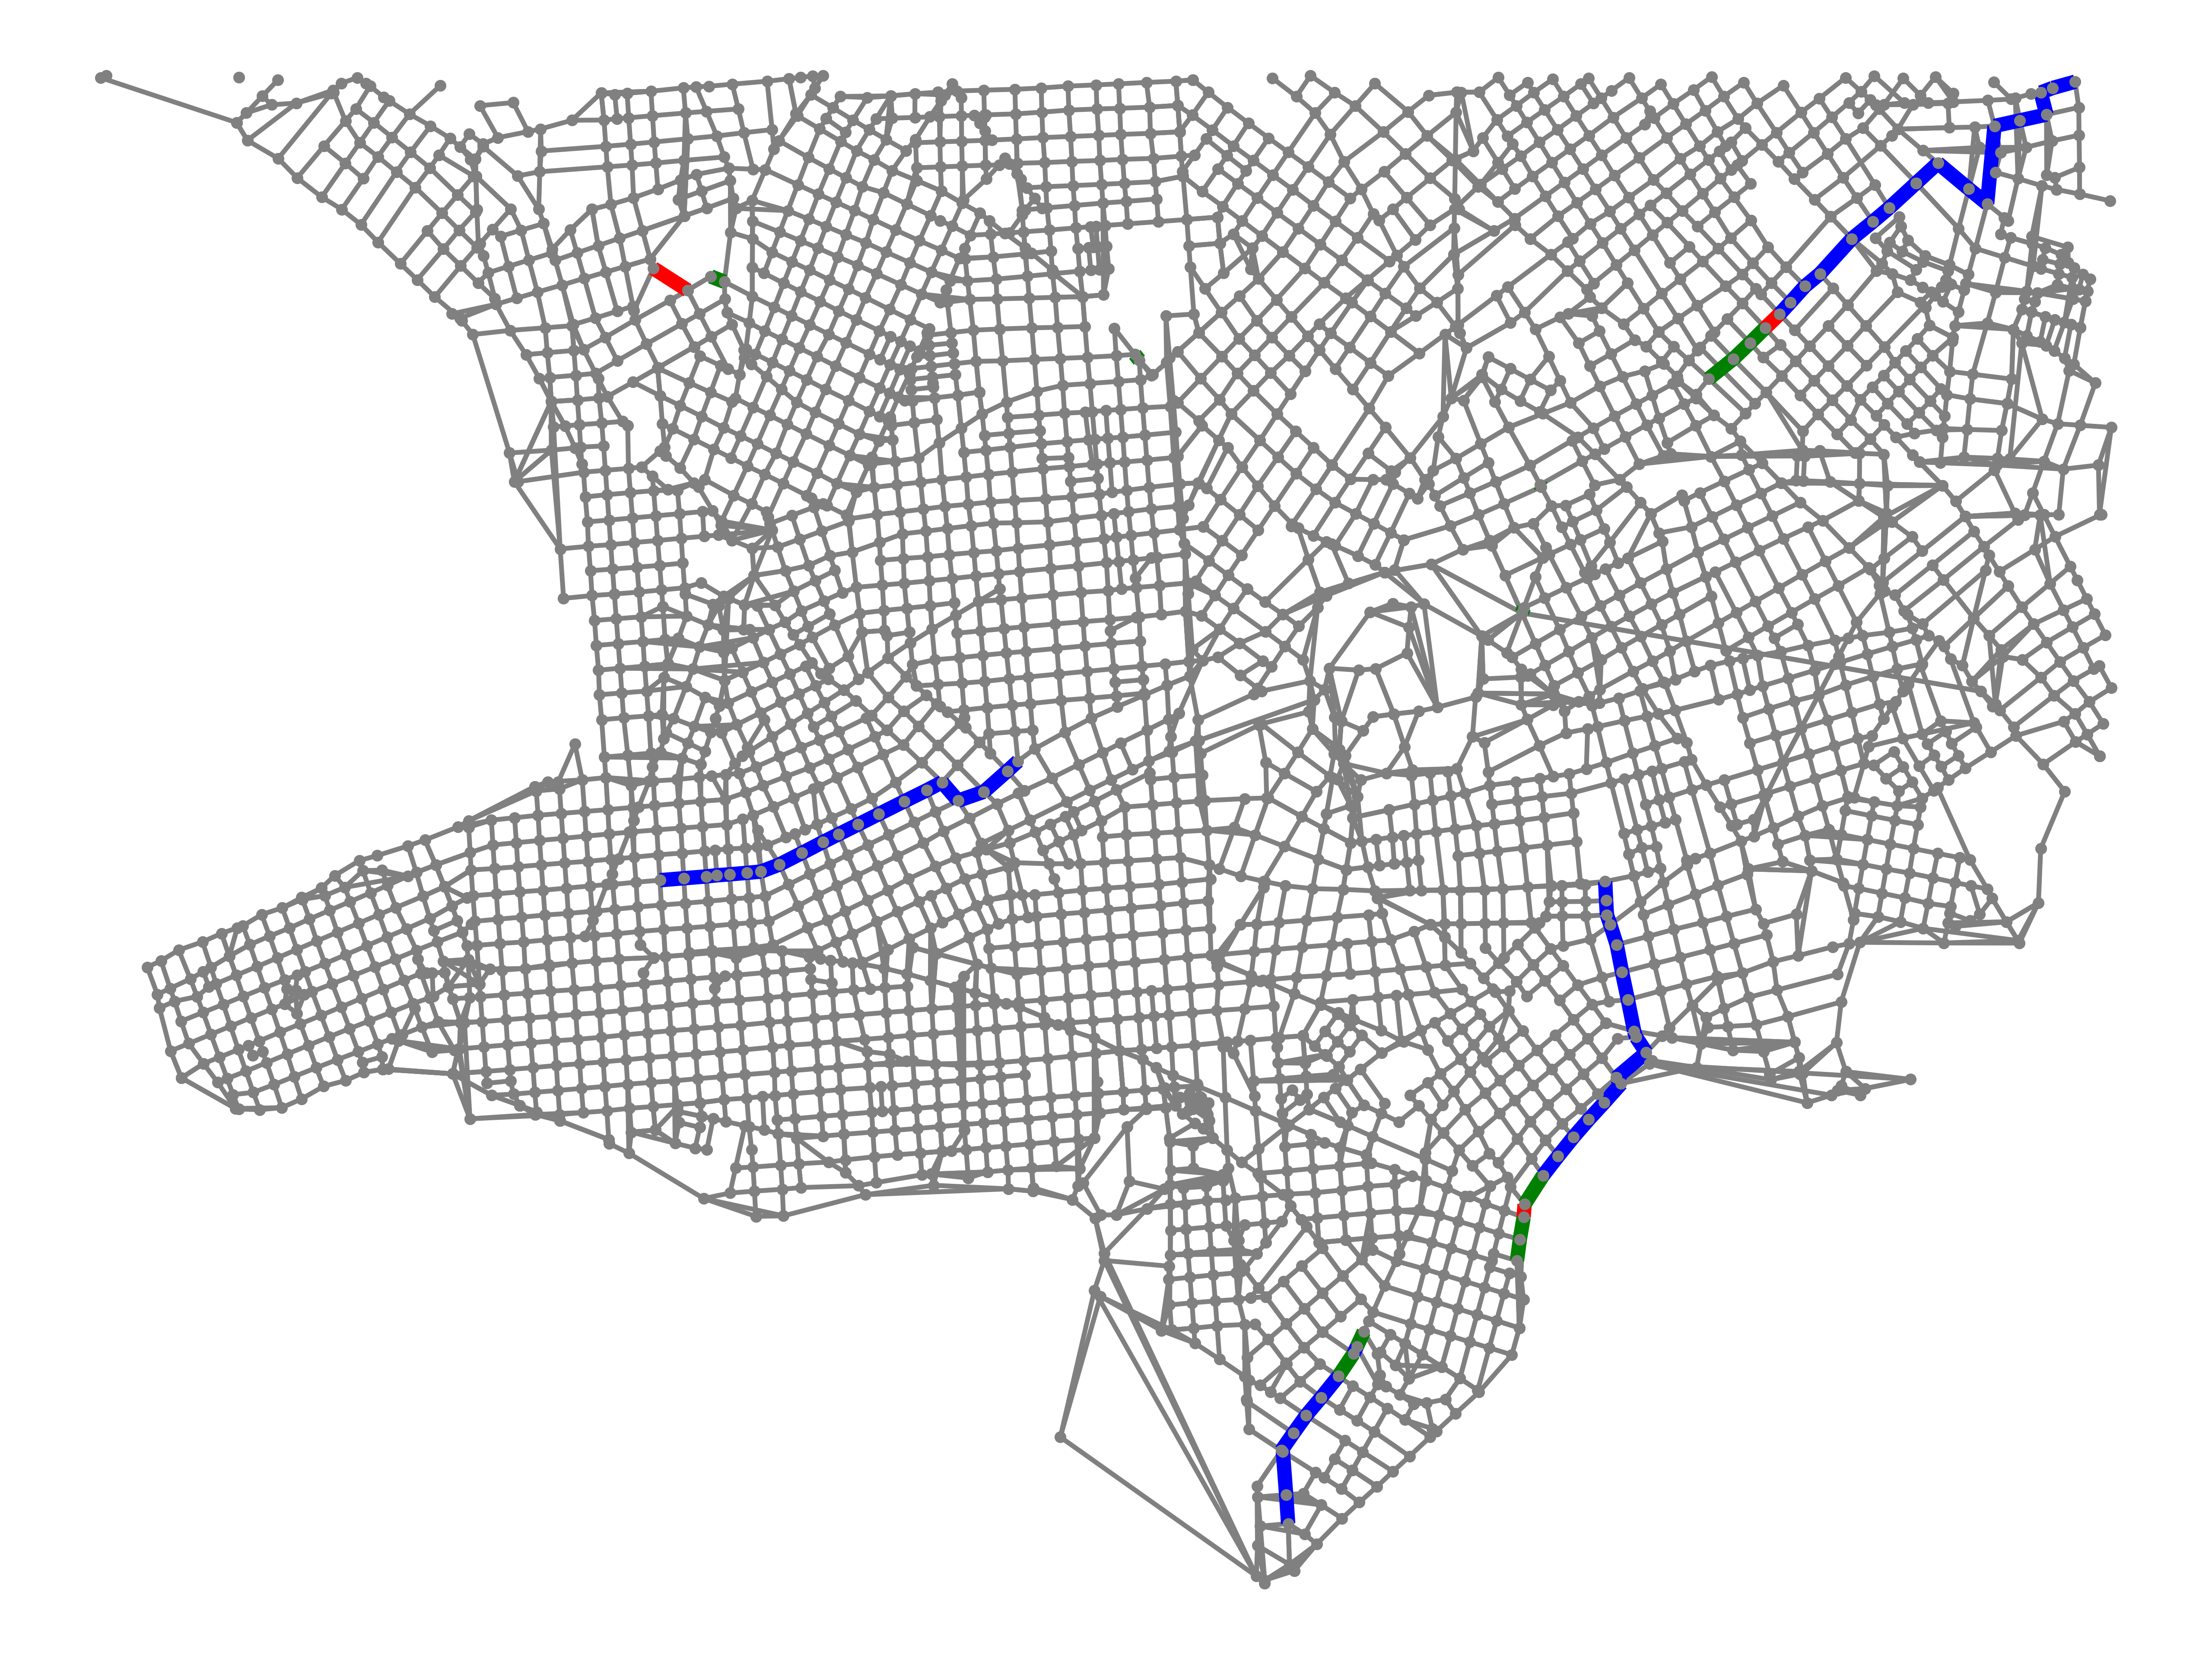
\includegraphics[width=10cm]{imgs/mdeo_large_pulse.png}
    \caption{Resultados de la ejecución del pulso para Montevideo. Los colores de las infraestructuras son: gris, verde, rojo y azul respectivamente al orden en que fueron definidas.}
    \label{resultadosmontevideo}
  \end{figure}

  \section*{Conclusión}

  Se mostró que el algorítmo del Pulso puede ser aplicado como metaheurístca del problema descrito. Si bien los resultados no fueron los mejores, hay mucho que se puede mejorar ya que esto solo fue una prueba de concepto de su aplicación.

  Hay varios caminos a seguir a partir de aquí. Se puede continuar con la mejora del algorítmo planteado en este trabajo o utilizarlo como pieza de otro sistema. Por ejemplo se podrían mejorar las soluciones de obtenidas por algún mecanismo de búsqueda local. En cualquier caso, vale la pena dedicar trabajo a futuras mejoras, algunas de las cuales se describen en la siguiente sección.

  \section*{Trabajo futuro}

  Este trabajo es una prueba de concepto que evidentemente puede ser mejorada y extendida. Aquí se detallan algunos puntos en este sentido.

  \subsection*{Forzar mejores soluciones por par origen-destino}

  El parámetro para configurar la ganancia sobre el costo base por par origen-destino debería ser configurado para cada par. El problema con la forma de dividir el presupuesto es que pueden haber pares origen-destino con muy poca demanda relativa al total, que por lo tanto no logran un asignación de presupuesto que permita obtener la ganancia impuesta por el parámetro. Esto puede causar que no exista solución para algún par origen-destino, lo que causa un infructuoso y largo tiempo de ejecución.

  \subsection*{Mejorar poda por costo}

  La poda por costo puede ser mejorada de manera que se poden pulsos mas tempranamente. La poda actual considera el cost bound multiplicado por un factor para obtener un costo proyectado hasta el destino. Sin embargo, el factor de multiplicación debería poder especificarse para cada par origen destino por un argumento similar al punto anterior. Dependiendo del presupuesto asignado, el costo proyectado debería ser mayor o menor.

  \subsection*{Mejora en la cola de pulsos}

  En cada iteración del algorítmo del Pulso, el pulso elegido es determinante para una buena y rápida convergencia. En el caso de Montevideo se tuvieron varios problemas en este aspecto por lo que un mejor diseño de esta lógica del algorítmo es clave.
  
  Por ejemplo se podrían considerar el costo de construcción junto al costo del pulso a insertar en la cola, para calcular el orden de ésta. Relacionado con el punto anterior, también se podría estimar el factor de multiplicación del cost bound dependiendo del valor de la restricción de presupuesto, de las infraestructuras disponibles y del costo del camino más corto.

  \subsection*{Incluir otras restricciones}

  El problema original cuenta con una restricción que no se contempló en este trabajo por simplicidad. La restricción es un límite inferior en la cantidad de infraestructuras consecutivas que se pueden construir, a excepción de la infraestructura base. Esto busca prevenir soluciones en las cuales las ciclovías cambian una y otra vez de infraestructura a lo largo de un recorrido.

  Esta restricción es interesante de implementar en el pulso ya que, a diferencia de la del presupuesto, es una restricción cota inferior y debe ser manejada de manera distinta en el chequeo de infactibilidad.

  \subsection*{Implementación más rápida}

  Para este estudio se utilizó python como lenguaje de implementación, que permite un desarrollo y puesta en funcionamiento rápidos pero no es tan bueno en términos de eficiencia en el cómputo. Una implementación en un lenguaje de más bajo nivel puede lograr mejoras considerables en el tiempo de ejecución.

  \subsection*{Version estocástica}

  Probar el mismo problema pero con una version estocástica del Pulso. Bastaría con cambiar la implementación de la cola de pulsos a una que utilice cierto grado de aleatoriedad.

  \subsection*{Versión paralela}

  Se puede analizar la posibilidad de paralelizar el Pulse solver. Por ejemplo correr un Pulso sobre una copia del multigrafo inicial para cada par origen-destino e ir generando un pool de caminos que luego el algorítmo recursivo va aplicando y adaptando según el estado del multigrafo dentro de la recursión.

  \section*{Implementación}

  La implementación de lo descrito en este trabajo se realizó en python y se encuentra accesible públicamente en el repositorio indicado la referencia \ref{repo}.

  Los principales directorios del repositorio son los siguientes:

  \begin{description}
    \item[/data]: Directorio que contiene los datos utilizados para correr los modelos. Aquí se encuentran los grafos utilizados (.yml), las configuraciones del Pulse solver (.json) y los archivos de datos de GLPK (.dat).
    \item[/exact]: Directorio que contiene el archivo de definición del modelo de GLPK. 
    \item[/proj]: Directorio donde se encuentra la implementación del pulso y del Pulse solver. En particular /proj/pulse/algo.py es donde se implementa el pulso. Y /proj/solver/solve.py es donde se implementa el solver.
  \end{description}

  Para ejecutar el Pulse solver, en la raíz del proyecto, se deben instalar las dependencias de python corriendo el comando pip install -r requirements.txt, luego se corre el pulse solver ejecutando, por ejemplo: ./bin/run instancia.json. Este comando ejecuta el solver utilizando los datos y la configuración especificada por el archivo instancia.json e imprime los resultados intermedios y finales a la salida estándar.

  \section*{Referencias}

  \begin{enumerate}
    \item{ \label{repo} \url{https://github.com/joaquinco/pulse-heuristic}}
  \end{enumerate}
\end{document}
